\section{Feature Engineering}
%
  \begin{figure}
    \centering
    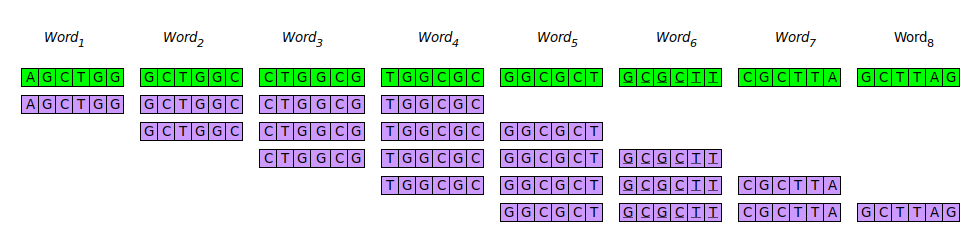
\includegraphics[scale=0.4]{ngrams}
    \caption{%
       4-word n-gram (\textit{4-gram}) phrases generated from 6-mer words representing the original nucleic acid sequence.
    }
    \label{fig:ngrams}
  \end{figure}
%
  \begin{figure}
    \centering
    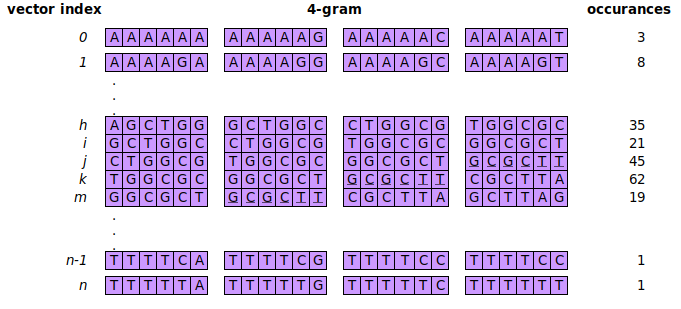
\includegraphics[scale=0.4]{count_vector}
    \caption{%
       4-word n-gram (\textit{4-gram}) phrases generated from 6-mer words representing the original nucleic acid sequence.
    }
    \label{fig:count-vector}
  \end{figure}
%

After converting contiguous nucleotide sequences into 6-mer words, \textit{Bag of Words} model was used to produce document vectors.


\subsection{n-grams}

We use CountVectorizer\footnote{\url{https://scikit-learn.org/stable/modules/generated/sklearn.feature_extraction.text.CountVectorizer.html}} to convert k-merized sequences to a matrix of token counts.

\autoref{fig:ngrams} above shows 4-gram phrases generated from a series of 6-mers of the original sequence. 
%
\subsection{Frequency Vectorization}
The frequencies of ordered 4-grams from each single nucleic acid k-merized sequence will produce a histogram based on the occurance of the 4-gram.
\autoref{fig:count-vector} above shows a Count Vector formed from 4-gram frequencies. 
%
